\begin{frame}{\tcii{} Policy search}
    \onslide<2->{
    \begin{center}
      \includegraphics[width=7cm]{images/misc/erl.png}\\
      \small \url{https://github.com/d9w/evolution/blob/master/imgs/erl.png}
    \end{center}
    }
\end{frame}

\begin{frame}{\tcii{} Neural networks}
    \begin{center}
      \includegraphics[width=8cm]{images/misc/dqn.png}\\
      \small Neural Network used in Deep Q Networks \cite{mnihHumanlevelControlDeep2015}
    \end{center}
\end{frame}

% \begin{frame}{\tcii{} \es}
%     \begin{center}
%       \includegraphics[width=6cm]{images/misc/es.png}\\
%       \small Evolution Strategy steps
%     \end{center}
% \end{frame}

\begin{frame}{\tcii{} \es}
    \begin{figure}

        \tikzset{every picture/.style={line width=0.75pt}} %set default line width to 0.75pt        

        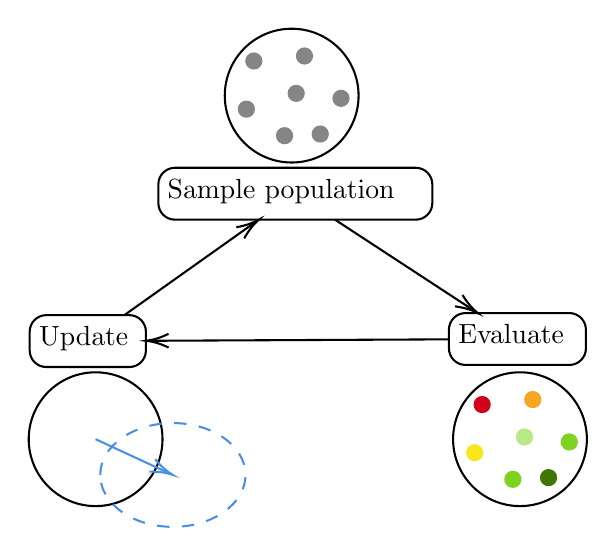
\begin{tikzpicture}[x=0.75pt,y=0.75pt,yscale=-1,xscale=1]
        %uncomment if require: \path (0,300); %set diagram left start at 0, and has height of 300
        \onslide<2->{
            %Shape: Circle [id:dp3485525204668506] 
            \draw  [draw opacity=0][fill={rgb, 255:red, 0; green, 0; blue, 0 }  ,fill opacity=0.48 ] (294.25,53.15) .. controls (294.25,50.86) and (296.11,49) .. (298.4,49) .. controls (300.69,49) and (302.55,50.86) .. (302.55,53.15) .. controls (302.55,55.44) and (300.69,57.29) .. (298.4,57.29) .. controls (296.11,57.29) and (294.25,55.44) .. (294.25,53.15) -- cycle ;
            %Shape: Circle [id:dp2866830478126762] 
            \draw  [draw opacity=0][fill={rgb, 255:red, 0; green, 0; blue, 0 }  ,fill opacity=0.48 ] (284.65,91.55) .. controls (284.65,89.26) and (286.51,87.4) .. (288.8,87.4) .. controls (291.09,87.4) and (292.95,89.26) .. (292.95,91.55) .. controls (292.95,93.84) and (291.09,95.69) .. (288.8,95.69) .. controls (286.51,95.69) and (284.65,93.84) .. (284.65,91.55) -- cycle ;
            %Shape: Circle [id:dp3451581426755682] 
            \draw  [draw opacity=0][fill={rgb, 255:red, 0; green, 0; blue, 0 }  ,fill opacity=0.48 ] (266.25,78.75) .. controls (266.25,76.46) and (268.11,74.6) .. (270.4,74.6) .. controls (272.69,74.6) and (274.55,76.46) .. (274.55,78.75) .. controls (274.55,81.04) and (272.69,82.89) .. (270.4,82.89) .. controls (268.11,82.89) and (266.25,81.04) .. (266.25,78.75) -- cycle ;
            %Shape: Circle [id:dp6444125122056538] 
            \draw  [draw opacity=0][fill={rgb, 255:red, 0; green, 0; blue, 0 }  ,fill opacity=0.48 ] (290.25,71.15) .. controls (290.25,68.86) and (292.11,67) .. (294.4,67) .. controls (296.69,67) and (298.55,68.86) .. (298.55,71.15) .. controls (298.55,73.44) and (296.69,75.29) .. (294.4,75.29) .. controls (292.11,75.29) and (290.25,73.44) .. (290.25,71.15) -- cycle ;
            %Shape: Circle [id:dp15892499220764567] 
            \draw  [draw opacity=0][fill={rgb, 255:red, 0; green, 0; blue, 0 }  ,fill opacity=0.48 ] (301.85,90.75) .. controls (301.85,88.46) and (303.71,86.6) .. (306,86.6) .. controls (308.29,86.6) and (310.15,88.46) .. (310.15,90.75) .. controls (310.15,93.04) and (308.29,94.89) .. (306,94.89) .. controls (303.71,94.89) and (301.85,93.04) .. (301.85,90.75) -- cycle ;
            %Shape: Circle [id:dp5122592703917728] 
            \draw  [draw opacity=0][fill={rgb, 255:red, 0; green, 0; blue, 0 }  ,fill opacity=0.48 ] (311.85,73.55) .. controls (311.85,71.26) and (313.71,69.4) .. (316,69.4) .. controls (318.29,69.4) and (320.15,71.26) .. (320.15,73.55) .. controls (320.15,75.84) and (318.29,77.69) .. (316,77.69) .. controls (313.71,77.69) and (311.85,75.84) .. (311.85,73.55) -- cycle ;
            %Shape: Circle [id:dp8859749705256629] 
            \draw  [draw opacity=0][fill={rgb, 255:red, 0; green, 0; blue, 0 }  ,fill opacity=0.48 ] (269.85,55.55) .. controls (269.85,53.26) and (271.71,51.4) .. (274,51.4) .. controls (276.29,51.4) and (278.15,53.26) .. (278.15,55.55) .. controls (278.15,57.84) and (276.29,59.69) .. (274,59.69) .. controls (271.71,59.69) and (269.85,57.84) .. (269.85,55.55) -- cycle ;
            %Shape: Circle [id:dp16165610575462575] 
            \draw   (260,72.23) .. controls (260,54.43) and (274.43,40) .. (292.23,40) .. controls (310.03,40) and (324.46,54.43) .. (324.46,72.23) .. controls (324.46,90.03) and (310.03,104.46) .. (292.23,104.46) .. controls (274.43,104.46) and (260,90.03) .. (260,72.23) -- cycle ;
            % Text Node
            \draw    (228,115) .. controls (228,110.58) and (231.58,107) .. (236,107) -- (352,107) .. controls (356.42,107) and (360,110.58) .. (360,115) -- (360,124) .. controls (360,128.42) and (356.42,132) .. (352,132) -- (236,132) .. controls (231.58,132) and (228,128.42) .. (228,124) -- cycle  ;
            \draw (231,111) node [anchor=north west][inner sep=0.75pt]   [align=left] {Sample population};
        }
        \onslide<3->{
            % Connection
            \draw    (313.11,132) -- (380.22,175.91) ;
            \draw [shift={(381.89,177)}, rotate = 213.19] [color={rgb, 255:red, 0; green, 0; blue, 0 }  ][line width=0.75]    (10.93,-3.29) .. controls (6.95,-1.4) and (3.31,-0.3) .. (0,0) .. controls (3.31,0.3) and (6.95,1.4) .. (10.93,3.29)   ;
            %Shape: Circle [id:dp24335528321652156] 
            \draw  [draw opacity=0][fill={rgb, 255:red, 245; green, 166; blue, 35 }  ,fill opacity=1 ] (404.25,218.69) .. controls (404.25,216.4) and (406.11,214.54) .. (408.4,214.54) .. controls (410.69,214.54) and (412.55,216.4) .. (412.55,218.69) .. controls (412.55,220.98) and (410.69,222.83) .. (408.4,222.83) .. controls (406.11,222.83) and (404.25,220.98) .. (404.25,218.69) -- cycle ;
            %Shape: Circle [id:dp8460877299146551] 
            \draw  [draw opacity=0][fill={rgb, 255:red, 126; green, 211; blue, 33 }  ,fill opacity=1 ] (394.65,257.09) .. controls (394.65,254.8) and (396.51,252.94) .. (398.8,252.94) .. controls (401.09,252.94) and (402.95,254.8) .. (402.95,257.09) .. controls (402.95,259.38) and (401.09,261.23) .. (398.8,261.23) .. controls (396.51,261.23) and (394.65,259.38) .. (394.65,257.09) -- cycle ;
            %Shape: Circle [id:dp7767476366344311] 
            \draw  [draw opacity=0][fill={rgb, 255:red, 248; green, 231; blue, 28 }  ,fill opacity=1 ] (376.25,244.29) .. controls (376.25,242) and (378.11,240.14) .. (380.4,240.14) .. controls (382.69,240.14) and (384.55,242) .. (384.55,244.29) .. controls (384.55,246.58) and (382.69,248.43) .. (380.4,248.43) .. controls (378.11,248.43) and (376.25,246.58) .. (376.25,244.29) -- cycle ;
            %Shape: Circle [id:dp9549751437175554] 
            \draw  [draw opacity=0][fill={rgb, 255:red, 184; green, 233; blue, 134 }  ,fill opacity=1 ] (400.25,236.69) .. controls (400.25,234.4) and (402.11,232.54) .. (404.4,232.54) .. controls (406.69,232.54) and (408.55,234.4) .. (408.55,236.69) .. controls (408.55,238.98) and (406.69,240.83) .. (404.4,240.83) .. controls (402.11,240.83) and (400.25,238.98) .. (400.25,236.69) -- cycle ;
            %Shape: Circle [id:dp7353313712102495] 
            \draw  [draw opacity=0][fill={rgb, 255:red, 65; green, 117; blue, 5 }  ,fill opacity=1 ] (411.85,256.29) .. controls (411.85,254) and (413.71,252.14) .. (416,252.14) .. controls (418.29,252.14) and (420.15,254) .. (420.15,256.29) .. controls (420.15,258.58) and (418.29,260.43) .. (416,260.43) .. controls (413.71,260.43) and (411.85,258.58) .. (411.85,256.29) -- cycle ;
            %Shape: Circle [id:dp10588540625648957] 
            \draw  [draw opacity=0][fill={rgb, 255:red, 126; green, 211; blue, 33 }  ,fill opacity=1 ] (421.85,239.09) .. controls (421.85,236.8) and (423.71,234.94) .. (426,234.94) .. controls (428.29,234.94) and (430.15,236.8) .. (430.15,239.09) .. controls (430.15,241.38) and (428.29,243.23) .. (426,243.23) .. controls (423.71,243.23) and (421.85,241.38) .. (421.85,239.09) -- cycle ;
            %Shape: Circle [id:dp49685818092818834] 
            \draw  [draw opacity=0][fill={rgb, 255:red, 208; green, 2; blue, 27 }  ,fill opacity=1 ] (379.85,221.09) .. controls (379.85,218.8) and (381.71,216.94) .. (384,216.94) .. controls (386.29,216.94) and (388.15,218.8) .. (388.15,221.09) .. controls (388.15,223.38) and (386.29,225.23) .. (384,225.23) .. controls (381.71,225.23) and (379.85,223.38) .. (379.85,221.09) -- cycle ;
            %Shape: Circle [id:dp23287136549655718] 
            \draw   (370,237.77) .. controls (370,219.97) and (384.43,205.54) .. (402.23,205.54) .. controls (420.03,205.54) and (434.46,219.97) .. (434.46,237.77) .. controls (434.46,255.57) and (420.03,270) .. (402.23,270) .. controls (384.43,270) and (370,255.57) .. (370,237.77) -- cycle ;
            % Text Node
            \draw    (368,185) .. controls (368,180.58) and (371.58,177) .. (376,177) -- (426,177) .. controls (430.42,177) and (434,180.58) .. (434,185) -- (434,194) .. controls (434,198.42) and (430.42,202) .. (426,202) -- (376,202) .. controls (371.58,202) and (368,198.42) .. (368,194) -- cycle  ;
            \draw (371,181) node [anchor=north west][inner sep=0.75pt]   [align=left] {Evaluate};
            }
            \onslide<4->{
                % Connection
                \draw    (211.61,178) -- (274.76,133.16) ;
                \draw [shift={(276.39,132)}, rotate = 144.63] [color={rgb, 255:red, 0; green, 0; blue, 0 }  ][line width=0.75]    (10.93,-3.29) .. controls (6.95,-1.4) and (3.31,-0.3) .. (0,0) .. controls (3.31,0.3) and (6.95,1.4) .. (10.93,3.29)   ;
            % Connection
            \draw    (368,189.66) -- (224,190.36) ;
            \draw [shift={(222,190.36)}, rotate = 359.72] [color={rgb, 255:red, 0; green, 0; blue, 0 }  ][line width=0.75]    (10.93,-3.29) .. controls (6.95,-1.4) and (3.31,-0.3) .. (0,0) .. controls (3.31,0.3) and (6.95,1.4) .. (10.93,3.29)   ;
            %Shape: Circle [id:dp39615038812496406] 
            \draw   (165.54,237.77) .. controls (165.54,219.97) and (179.97,205.54) .. (197.77,205.54) .. controls (215.57,205.54) and (230,219.97) .. (230,237.77) .. controls (230,255.57) and (215.57,270) .. (197.77,270) .. controls (179.97,270) and (165.54,255.57) .. (165.54,237.77) -- cycle ;
            %Shape: Ellipse [id:dp023503223261750472] 
            \draw  [color={rgb, 255:red, 74; green, 144; blue, 226 }  ,draw opacity=1 ][dash pattern={on 4.5pt off 4.5pt}] (200,255) .. controls (200,241.19) and (215.67,230) .. (235,230) .. controls (254.33,230) and (270,241.19) .. (270,255) .. controls (270,268.81) and (254.33,280) .. (235,280) .. controls (215.67,280) and (200,268.81) .. (200,255) -- cycle ;
            %Straight Lines [id:da6417213751784759] 
            \draw [color={rgb, 255:red, 74; green, 144; blue, 226 }  ,draw opacity=1 ]   (197.77,237.77) -- (233.18,254.16) ;
            \draw [shift={(235,255)}, rotate = 204.83] [color={rgb, 255:red, 74; green, 144; blue, 226 }  ,draw opacity=1 ][line width=0.75]    (10.93,-3.29) .. controls (6.95,-1.4) and (3.31,-0.3) .. (0,0) .. controls (3.31,0.3) and (6.95,1.4) .. (10.93,3.29)   ;
            % Text Node
            \draw    (166,186) .. controls (166,181.58) and (169.58,178) .. (174,178) -- (214,178) .. controls (218.42,178) and (222,181.58) .. (222,186) -- (222,195) .. controls (222,199.42) and (218.42,203) .. (214,203) -- (174,203) .. controls (169.58,203) and (166,199.42) .. (166,195) -- cycle  ;
            \draw (169,182) node [anchor=north west][inner sep=0.75pt]   [align=left] {Update};
        }
        
        \end{tikzpicture}
        

    \end{figure}
\end{frame}


\begin{frame}{\tcii{} Variants of \es}
    \onslide<1->{
    \begin{block}{Evolution Strategies}
        \begin{columns}
            \begin{column}{0.45\linewidth}
                \begin{itemize}
                    \item ($\mu , \lambda$) ES
                    \item \snes
                    \item Canonical ES 
                    \item OpenAI ES
                \end{itemize}
            \end{column}
            \begin{column}{0.45\linewidth}
                \begin{itemize}
                    \item \cmaes
                    \item \xnes
                    \item Cross-Entropy Method
                    \item Augmented Random Search
                \end{itemize}
            \end{column}
        \end{columns}
    \end{block}
    }
    \onslide<2->{   
    \begin{block}{Neuroevolution for policy search}
        \begin{itemize}
            \item large dimensions (1.6 $.10^6$ parameters)
            \item expensive evaluation 
        \end{itemize}
    \end{block}
    }
    
\end{frame}

\begin{frame}{\tcii{} Benchmarking Evolutionary Reinforcement Learning}

    \begin{block}{Reproduction settings}
        Reproducing \canonical{} \canonicalpaper{} and \openaies{} \openaipaper{} on the Arcade Learning Environment.
    \end{block}
    
    \begin{center}
        \begin{figure}
            \includegraphics[width=7cm]{images/BERL/Alien-v0.png}
            \caption{Evolution of \canonical{} and \openaies{} on Alien with 800 CPUh compute budget}
        \end{figure}
    \end{center}

\end{frame}